\chapter{Methodology and Implementation}
\label{chap:implementation}
 
In this chapter the implementation of the GraphSLAM algorithm is presented and explained. The implementation created is capable of solving the SLAM problem in an offline manner for a 2D scenario, in the cases of known and unknown data association.

The g$^2$o framework used in this work provides of a least squares solver for the optimization of equation~\eqref{eq:minimization}, as well as a protocol to define a graph in the SLAM problem. g$^2$o is well optimized and it has several options for the solver, so the known correspondence version of the GraphSLAM algorithm is relative straightforward to implement.

However, g$^2$o doesn't provide a way to handle unknown data association, so the main goal of this work is to implement a method for solving the correspondence problem in an efficient manner.

\section{g$^2$o Protocol}

The first step to implementing the GraphSLAM algorithm is to define a protocol to store and interpret the data on a graph. g$^2$o already provides such protocol. The stored data comes in two types: data from nodes, and data from edges. 

In SLAM context, nodes itself can be of two types, pose nodes and landmark nodes. Pose nodes represent the pose of the robot, in the 2D case they consists in 3 variables: robot's $x$ and $y$ position, and robot's bearing $\theta$. In g$^2$o a pose node is denoted with the keyword \texttt{VERTEX\_SE2}\footnote{Vertex is synonymous of node. SE2 is the Non-Euclidean space that consists of two spatial dimensions and a angular dimension.}. Landmark nodes represent the 2D position ($x$ and $y$) of a landmark. They are denoted with the keyword \texttt{VERTEX\_XY}.

Edges represents either robot's odometry (data of robot's change in position), or robot's measurements of landmarks. Odometry is measured as the difference between robot's pose at two consecutive timesteps: $(\Delta x, \Delta y, \Delta \theta)$. On the other hand, robot measurement are given as the $x$ and $y$ distance to the landmark relative to the robot reference frame. Figure~\ref{fig:protocol} illustrates the odometry an measurement of a robot. Keywords \texttt{EDGE\_SE2} and \texttt{EDGE\_SE2\_XY} are use to denote odometry and measurement edges respectively.

\begin{figure}[htbp!]
    \centering
    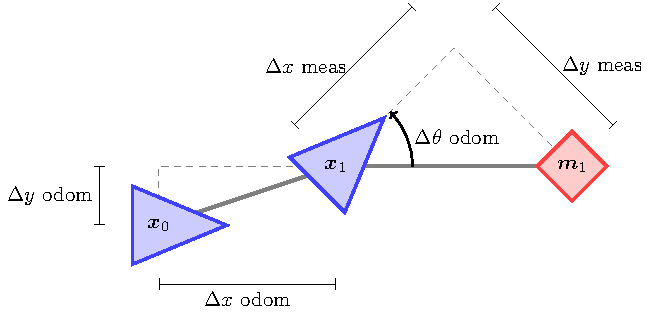
\includegraphics[width=0.7\textwidth]{tikz/protocol.pdf}
    \caption{Ilustration of odometry and measurements values in g$^2$o.}
    \label{fig:protocol}
\end{figure}

For GraphSLAM to work correctly, one must also provide to the algorithm of the uncertainty of odometry and measurements. These correspond to the covariance matrices $\bs{R}_k$ and $\bs{Q}_k$ from motion~\eqref{eq:motion-model} and measurement~\eqref{eq:measurement-model} model respectively. Actually g$^2$o works with the inverse of the covariance matrix, known as the information matrix, however, these representation are equivalent in terms of the knowledge of the system. Since covariance matrices (and their inverse) are symmetrical, only the upper diagonal elements are needed. In this work it is assumed that the model's uncertainly are time independent, i.e., all nodes have the same values for the information matrix. The notation of each element of the matrices is shown as follows:

\begin{equation}
    \bs{R}^{-1}_k = \begin{pmatrix}
    ipxx & ipxy & ipxt\\
    ipxy & ipyy & ipyt\\
    ipxt & ipyt & iptt
    \end{pmatrix} \;\;
    \bs{Q}^{-1}_k = \begin{pmatrix}
    ilxx & ilxy\\
    ilxy & ilyy
    \end{pmatrix} 
\end{equation}

Finally, nodes must be indexed so they can be distinguishable form other nodes, indicated by an integer \texttt{id}. Ids are used in edges to indicate the two nodes that the edge is connecting.

Table~\ref{tab:protocol} summarize the g$^2$o notation to represent nodes and edges:

\begin{table}[htbp!]
    \centering
    \begin{tabular}{|c|c|}
        \hline
        Graph element & Notation\\
        \hline
        Pose node & \texttt{VERTEX\_SE2 id x y t}\\
        Landmark node & \texttt{VERTEX\_SE2\_XY id x y}\\
        Odometry edge & \texttt{EDGE\_SE2 id1 id2 dx dy dt ipxx ipxy ipxt ipyy ipyt ipyy}\\
        Measurement edge & \texttt{EDGE\_SE2\_XY id1 id2 dx dy ilxx ilxy ilyy}\\
        \hline
    \end{tabular}
    \caption{g$^2$o protocol for node and edge definition.}
    \label{tab:protocol}
\end{table}

In a SLAM problem one usually have only information about robot odometry and measurement, so only edges data is known. All the data can be written in a plain text, that can be latter uploaded to the g$^2$o framework.

\section{The Known Correspondence Case}

\section{The Unknown Correspondence Case}
